\documentclass[border=10pt]{standalone}
\usepackage{tikz}
\usetikzlibrary{shapes,backgrounds,calc,patterns,trees}

\begin{document}
	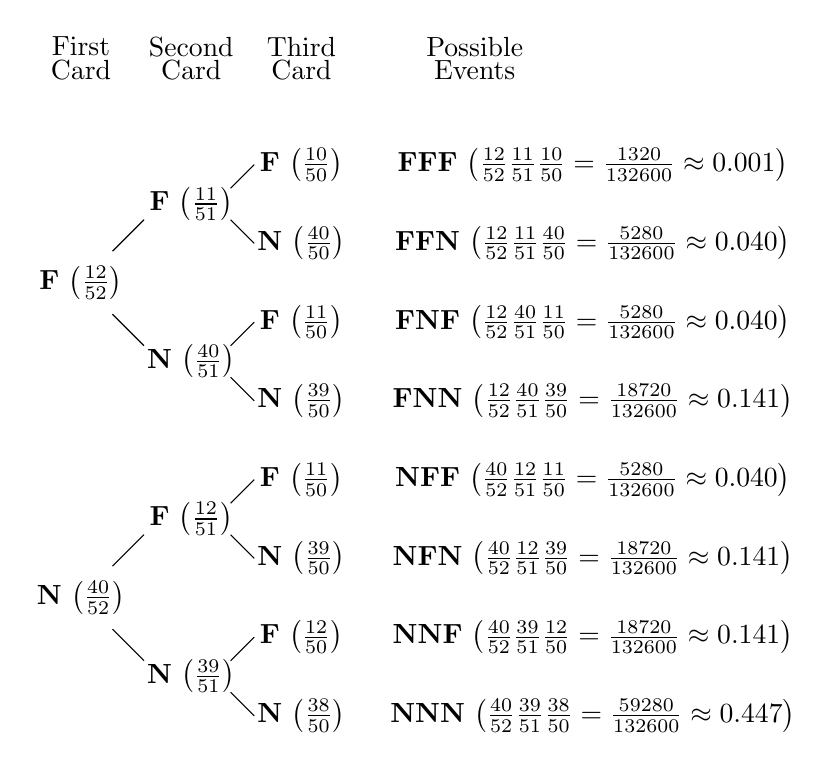
\begin{tikzpicture}
		\node at (0,5) {First};
		\node at (0,4.7) {Card};
		
		
		\node at (1.4,5) {Second};
		\node at (1.4,4.7) {Card};
		
		\node at (2.8, 5) {Third};
		\node at (2.8, 4.7) {Card};
		
		
		\node at (5,5) {Possible};
		\node at (5, 4.7) {Events};



		\node at (0,2) {\textbf{F} \(\left(\frac{12}{52}\right)\)};
		
		\draw (.4,2.4) -- (.8,2.8);
		\draw (.4,1.6) -- (.8,1.2);
		
			\node at (1.4,3) {\textbf{F} \(\left(\frac{11}{51}\right)\)};
			
				\draw (1.9,3.2) -- (2.2,3.5);
				\draw (1.9,2.8) -- (2.2,2.5);
			
				\node at (2.8, 3.5) {\textbf{F} \(\left(\frac{10}{50}\right)\)};
				
				\node at (2.8, 2.5) {\textbf{N} \(\left(\frac{40}{50}\right)\)};
		
			\node at (1.4,1) {\textbf{N} \(\left(\frac{40}{51}\right)\)};
			
				\draw (1.9,.8) -- (2.2,.5) ;
				\draw (1.9,1.2) -- (2.2,1.5);
			
				\node at (2.8,1.5) {\textbf{F} \(\left( \frac{11}{50}\right)\)};
				
				\node at (2.8,.5) {\textbf{N} \(\left( \frac{39}{50}\right)\)};
		
		
		
		\node at (0,-2) {\textbf{N} \(\left(\frac{40}{52}\right)\)};
		
				\draw (.4,-2.4) -- (.8,-2.8);
				\draw (.4,-1.6) -- (.8,-1.2);
		
	
				\node at (1.4,-1) {\textbf{F} \(\left(\frac{12}{51}\right)\)};
				
					\draw (1.9,-.8) -- (2.2,-.5) ;
					\draw (1.9,-1.2) -- (2.2,-1.5);
				
					\node at (2.8,-1.5) {\textbf{N} \(\left( \frac{39}{50}\right)\)};
				
					\node at (2.8,-.5) {\textbf{F} \(\left( \frac{11}{50}\right)\)};
	
				\node at (1.4,-3) {\textbf{N} \(\left(\frac{39}{51}\right)\)};
					
					\draw (1.9,-3.2) -- (2.2,-3.5);
					\draw (1.9,-2.8) -- (2.2,-2.5);
				
				\node at (2.8,-3.5) {\textbf{N} \(\left(\frac{38}{50}\right)\)};
				
				\node at (2.8,-2.5) {\textbf{F} \(\left(\frac{12}{50}\right)\)};
		
		\node at (6.5,3.5) {\textbf{FFF} \(\left( \frac{12}{52} \frac{11}{51} \frac{10}{50} = \frac{1320}{132600} \approx 0.001 \right)\)};		

		\node at (6.5,2.5) {\textbf{FFN} \(\left( \frac{12}{52} \frac{11}{51} \frac{40}{50} = \frac{5280}{132600} \approx 0.040 \right)\)};	
		
		\node at (6.5,1.5) {\textbf{FNF} \(\left( \frac{12}{52} \frac{40}{51} \frac{11}{50} = \frac{5280}{132600} \approx 0.040 \right)\)};
		
		\node at (6.5,.5) {\textbf{FNN} \(\left( \frac{12}{52} \frac{40}{51} \frac{39}{50} = \frac{18720}{132600} \approx 0.141 \right)\)};
		
		\node at (6.5,-.5) {\textbf{NFF} \(\left( \frac{40}{52} \frac{12}{51} \frac{11}{50} = \frac{5280}{132600} \approx 0.040 \right)\)};
		
		\node at (6.5,-1.5) {\textbf{NFN} \(\left( \frac{40}{52} \frac{12}{51} \frac{39}{50} = \frac{18720}{132600} \approx 0.141 \right)\)};
		
		\node at (6.5,-2.5) {\textbf{NNF} \(\left( \frac{40}{52} \frac{39}{51} \frac{12}{50} = \frac{18720}{132600} \approx 0.141 \right)\)};
		
		\node at (6.5,-3.5) {\textbf{NNN} \(\left( \frac{40}{52} \frac{39}{51} \frac{38}{50} = \frac{59280}{132600} \approx 0.447 \right)\)};			
	
	\end{tikzpicture}
\end{document}

